\iffalse
\documentclass[12pt]{article}
\usepackage{graphicx}
\usepackage{amsmath}   % for having text in math mode

%Following 2 lines were added to remove the blank page at the beginning
\usepackage{atbegshi}% http://ctan.org/pkg/atbegshi
\AtBeginDocument{\AtBeginShipoutNext{\AtBeginShipoutDiscard}}
%

\begin{document}

\begin{center}
\title{\textbf{Area of a Traingle}}
\date{\vspace{-5ex}} %Not to print date automatically
\maketitle
\end{center}

\setcounter{page}{1}



\section{10$^{th}$ Maths - Chapter 7}

All problems are from Exercise 7.3

\fi
%\begin{enumerate}[label=\thechapter.\arabic*,ref=\thechapter.\theenumi]
\begin{enumerate}[label=\thesection.\arabic*,ref=\thesection.\theenumi]
\numberwithin{equation}{enumi}
\numberwithin{figure}{enumi}
\numberwithin{table}{enumi}
\item Find the area of the triangle whose vertices are 
\begin{enumerate}
\item $(2, 3), (–1, 0), (2, – 4)$
\item $(–5, –1), (3, –5), (5, 2)$ 
\end{enumerate}
		\label{10/7/3/1}
\solution
		\iffalse
\documentclass[12pt]{article}
\usepackage{graphicx}
%\documentclass[journal,12pt,twocolumn]{IEEEtran}
\usepackage[none]{hyphenat}
\usepackage{graphicx}
\usepackage{listings}
\usepackage[english]{babel}
\usepackage{graphicx}
\usepackage{caption} 
\usepackage{hyperref}
\usepackage{booktabs}
\usepackage{array}
\usepackage{amsmath}   % for having text in math mode

%Following 2 lines were added to remove the blank page at the beginning
\usepackage{atbegshi}% http://ctan.org/pkg/atbegshi
\AtBeginDocument{\AtBeginShipoutNext{\AtBeginShipoutDiscard}}
%


%New macro definitions
\newcommand{\mydet}[1]{\ensuremath{\begin{vmatrix}#1\end{vmatrix}}}
\providecommand{\brak}[1]{\ensuremath{\left(#1\right)}}
\providecommand{\norm}[1]{\left\lVert#1\right\rVert}
\newcommand{\solution}{\noindent \textbf{Solution: }}
\newcommand{\myvec}[1]{\ensuremath{\begin{pmatrix}#1\end{pmatrix}}}
\let\vec\mathbf

\begin{document}

\begin{center}
\title{\textbf{Area of a Traingle}}
\date{\vspace{-5ex}} %Not to print date automatically
\maketitle
\end{center}

\setcounter{page}{1}



\section{10$^{th}$ Maths - Chapter 7}

This is Problem-1 from Exercise 7.3

\begin{enumerate}
\item Find the area of the triangle whose vertices are :
	\fi
\begin{enumerate}
\item 
In this case, the area  is given by  
  \label{prop:10/7/3/1area2d}
  \begin{align}
    \label{eq:10/7/3/1area2d}
	\frac{1}{2}\norm{\brak{\vec{A}-\vec{B}} \times \brak{\vec{A}-\vec{C}}} \\
  \end{align}
  Since
  \begin{align}
	 \vec{A}-\vec{B} =  \myvec{
  2 \\
  3 \\
 } - \myvec{
  -1 \\
  0 \\
 } = \myvec{
 3 \\
 3 \\
 }
 \\
 \vec{A}-\vec{C} =  \myvec{
  2 \\
  3 \\
 } - \myvec{
  2 \\
  -4 \\
 } = \myvec{
 0 \\
 7 \\
 }
 \end{align}
 the desired area is given by 
 \iffalse
The value of the cross product of two vectors is given by
\begin{align}
  \label{eq:10/7/3/1det2d}
  \mydet{\vec{M}} &= \mydet{\vec{A} & \vec{B}} 
  \\
  &= \mydet{a_1 & b_1\\a_2 & b_2} = a_1b_2 - a_2 b_1
\end{align}

		Therefore, \eqref{eq:10/7/3/1area2d} equals \\
		\fi
\begin{align}
	\frac{1}{2}\mydet{3 & 0\\3 & 7}  
	&=	\frac{21}{2}
\end{align}
\iffalse
\begin{figure}[!h]
	\begin{center}
		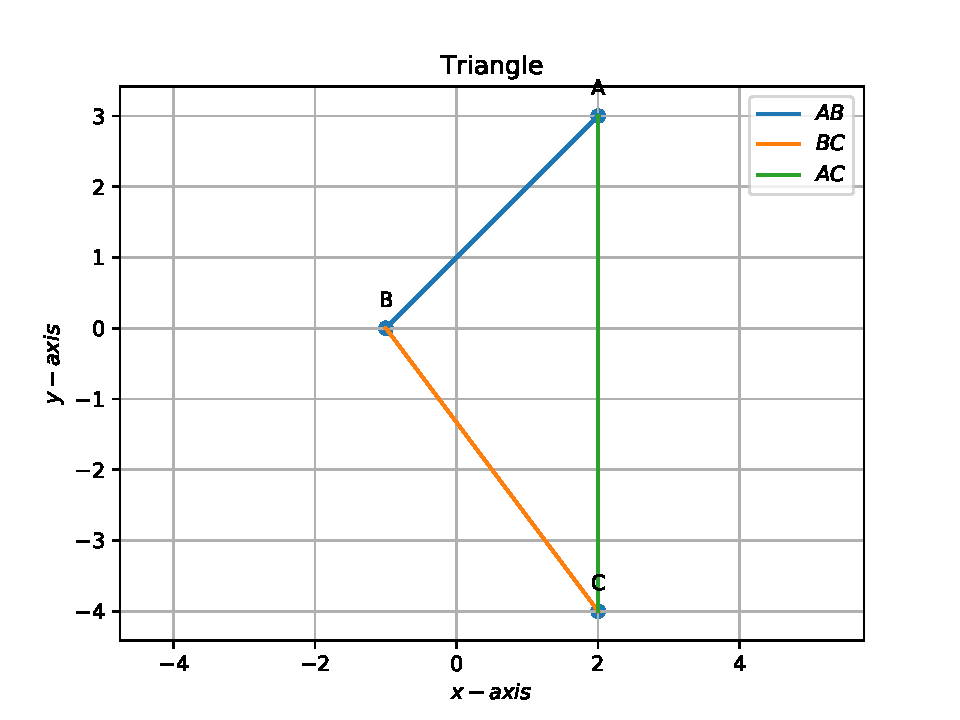
\includegraphics[width=\columnwidth]{./figs/problem1a.pdf}
	\end{center}
\caption{}
\label{fig:Fig1}
\end{figure}
\fi

\item In this case, 
	\iffalse
\solution The area of the triangle with vertices $\vec{A}, \vec{B}, \vec{C}$ is given by  
  \label{prop:10/7/3/1area2e}
  \begin{align}
    \label{eq:10/7/3/1area2e}
	\frac{1}{2}\norm{\brak{\vec{A}-\vec{B}} \times \brak{\vec{A}-\vec{C}}} \\
	\fi
  \begin{align}
	 \vec{A}-\vec{B} =  \myvec{
  -5 \\
  -1 \\
 } - \myvec{
  3 \\
  -5 \\
 } = \myvec{
 -8 \\
 4 \\
 }
 \\
 \vec{A}-\vec{C} =  \myvec{
  -5 \\
  -1 \\
 } - \myvec{
  5 \\
  2 \\
 } = \myvec{
 -10 \\
 -3 \\
 }
 \\
	  \implies
\text{Area} =	\frac{1}{2}\mydet{-8 & -10\\4 & -3}  
	=  32 
\end{align}
\iffalse
\begin{figure}[!h]
	\begin{center}
		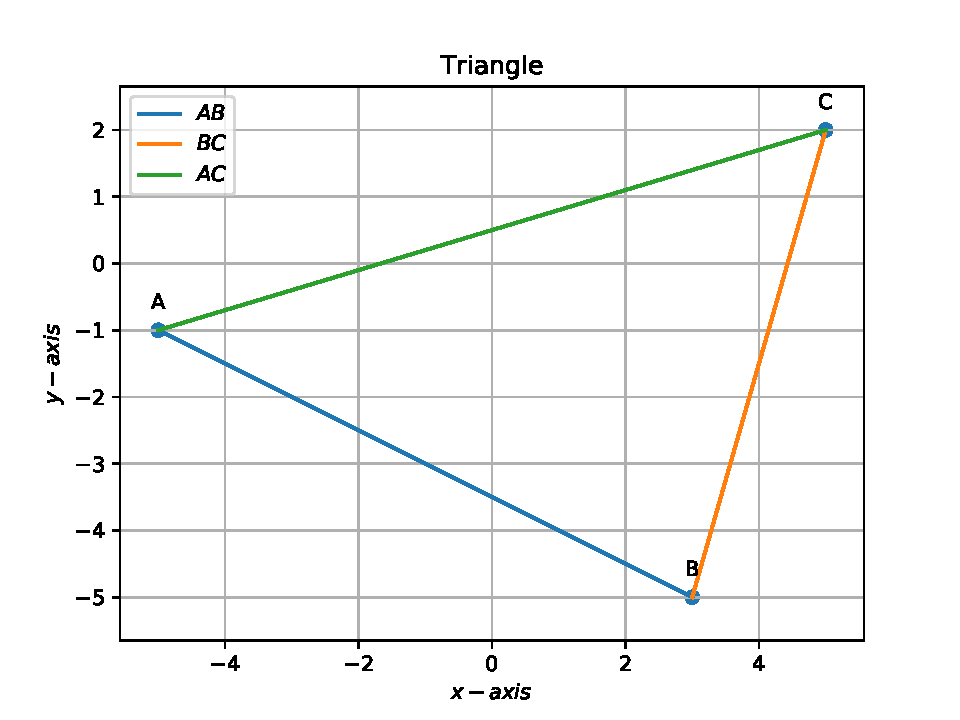
\includegraphics[width=\columnwidth]{./figs/problem1b.pdf}
	\end{center}
\caption{}
\label{fig:Fig2}
\end{figure}
\fi
\end{enumerate}




\item In each of the following, find the value of '$k$', for which the points are collinear.
\begin{enumerate}
\item $(7, –2), (5, 1), (3, k)$
\item $(8, 1), (k, – 4), (2, –5)$
\end{enumerate}
		\label{10/7/3/2}
\solution
		\iffalse
\documentclass[journal,12pt,twocolumn]{IEEEtran}
\usepackage{graphicx}
\graphicspath{{./figs/}}{}
\usepackage{amsmath,amssymb,amsfonts,amsthm}
\newcommand{\myvec}[1]{\ensuremath{\begin{pmatrix}#1\end{pmatrix}}}
\providecommand{\norm}[1]{\lVert#1\rVert}
\usepackage{listings}
\usepackage{watermark}
\usepackage{titlesec}
\usepackage{caption}
\usepackage{enumitem}
\usepackage{extarrows}
\let\vec\mathbf
\lstset{
frame=single, 
breaklines=true,
columns=fullflexible
}
\thiswatermark{\centering \put(0,-105.0){
\includegraphics[scale=0.15]{/sdcard/IITH/vector/vector-3/figs/logo.png}} }
\title{\mytitle}
\title{
Assignment - Vector-3
}
\author{Surajit Sarkar}
\begin{document}
\maketitle
\tableofcontents
\bigskip
\section{\textbf{Problem}}
In each of the following, find the value of ’k’,\\ for which the points are collinear.
\begin{enumerate}[label=(\roman*)]
\item (7, –2), (5, 1), (3, k)
\item(8, 1), (k, –4), (2, –5)
\end{enumerate}
\section{\textbf{Solution}}
\fi
\begin{enumerate}
    \item Given
    \begin{align}
      \vec{A}=\myvec{7\\-2},\Vec{B}=\myvec{5\\1},\vec{C}=\myvec{3\\k}  
    \end{align}
    Then
    \begin{align}
        \myvec{\vec{A}-\vec{B}}&=\myvec{2\\-3}\\
        \myvec{\vec{A}-\vec{C}}&=\myvec{4\\2k}\
    \end{align}
    Forming the collinearity matrix
    \begin{align}
        \myvec{2&-3\\4&2k} \xleftrightarrow{R_1\rightarrow{R_1-1}}&\myvec{1&-2\\4&2k}\\
         \xleftrightarrow{R_1\rightarrow{R_1-1}}&\myvec{1&-2\\0&2k+8}\\
        k&=4
        \end{align}
    
    \item Given
     \begin{align}
      \vec{A}=\myvec{8\\1},\vec{B}=\myvec{k\\-4},\vec{C}=\myvec{2\\-5}  
    \end{align}
    Then
    \begin{align}
        \myvec{\vec{A}-\vec{B}}&=\myvec{-8k\\-5}\\
        \myvec{\vec{A}-\vec{C}}&=\myvec{6\\6}\
    \end{align}
    Forming the collinearity matrix
    \begin{align}
        \myvec{-8-k&-5\\6&6} \xleftrightarrow{R_1\rightarrow{R_1+8}}&\myvec{-k&3\\6&6}\\
        k&=3
        \end{align}
\end{enumerate}



\item Find the area of the triangle formed by joining the mid-points of the sides of the triangle whose vertices are $(0, –1), (2, 1) \text{ and } (0, 3)$. Find the ratio of this area to the area of the given triangle.
	\\
\solution
		\iffalse
\documentclass[12pt]{article}
\usepackage{graphicx}
\usepackage{amsmath}
\usepackage{mathtools}
\usepackage{gensymb}

\newcommand{\mydet}[1]{\ensuremath{\begin{vmatrix}#1\end{vmatrix}}}
\providecommand{\brak}[1]{\ensuremath{\left(#1\right)}}
\providecommand{\norm}[1]{\left\lVert#1\right\rVert}
\newcommand{\solution}{\noindent \textbf{Solution: }}
\newcommand{\myvec}[1]{\ensuremath{\begin{pmatrix}#1\end{pmatrix}}}
\let\vec\mathbf

\begin{document}
\begin{center}
\textbf\large{CHAPTER-7 \\ COORDINATE GEOMETRY}
\end{center}
\section*{Excercise 7.2}

Q3. Find the area of the triangle formed by joining the mid-points of the sides of the triangle
whose vertices are $\vec(0, –1), \vec(2, 1) \text{ and } \vec(0, 3)$. Find the ratio of this area to the area of the
given triangle
\\
\solution
\\
\fi
The coordinates are given as
	\begin{align}
	\vec{A} = \myvec{
		0\\
		-1\\
		},
	\vec{B} = \myvec{
		2\\
		1\\
		},
	\vec{C} = \myvec{
		0\\
		3\\
		}
	\end{align}
Calculating midpoints,
	\begin{align}
		\vec{P} = \frac{1}{2}\vec(\vec{A}+\vec{B}) = \frac{1}{2}\myvec{2\\0\\} = \myvec{1\\0\\}\\
		\vec{Q} = \frac{1}{2}\vec(\vec{B}+\vec{C}) = \frac{1}{2}\myvec{2\\4\\} = \myvec{1\\2\\}\\
		\vec{R} = \frac{1}{2}\vec(\vec{A}+\vec{C}) = \frac{1}{2}\myvec{0\\2\\} = \myvec{0\\1\\}
	\end{align}
	Since
	\begin{align}
		\vec{P}-\vec{Q} &=  \myvec{
  1 \\
  0 
 } - \myvec{
  1 \\
  2 
 } = \myvec{
 0 \\
 -2 
 }
		\\
		\vec{Q}-\vec{R} &=  \myvec{
  1 \\
  2 \\
 } - \myvec{
  0 \\
  1 \\
 } = \myvec{
 1 \\
 1 \\
 }
	\end{align}
	the area is obtained as
	\begin{align}
		ar(PQR)&=\frac{1}{2}{\norm{\vec(\vec{P}-\vec{Q})\times\vec(\vec{Q}-\vec{R})}}
		\\
		&=\frac{1}{2}\mydet{0 & 1\\-2 & 1}
		=1
	\end{align}
	Similarly, 
	\begin{align}
		\vec{A}-\vec{B} &=  \myvec{
  0 \\
  -1 \\
 } - \myvec{
  2 \\
  1 \\
 } = \myvec{
 -2 \\
 -2 \\
 }
 \\
		\vec{A}-\vec{C} &=  \myvec{
  0 \\
  -1 \\
 } - \myvec{
  0 \\
  3 \\
 } = \myvec{
 0 \\
 -4 \\
 }
	\end{align}
 the area is obained as
	\begin{align}
		ar(ABC)&=\frac{1}{2}{\norm{\vec(\vec{A}-\vec{B})\times\vec(\vec{A}-\vec{C})}}\\
		&=\frac{1}{2}\mydet{-2 & 0\\-2 & -4}
=4
	\end{align}
	Thus, the resultant ratio of two areas is 1:4.
	See Fig.
\ref{fig:10/7/3/3Fig}
\begin{figure}[!h]
	\begin{center} 
	    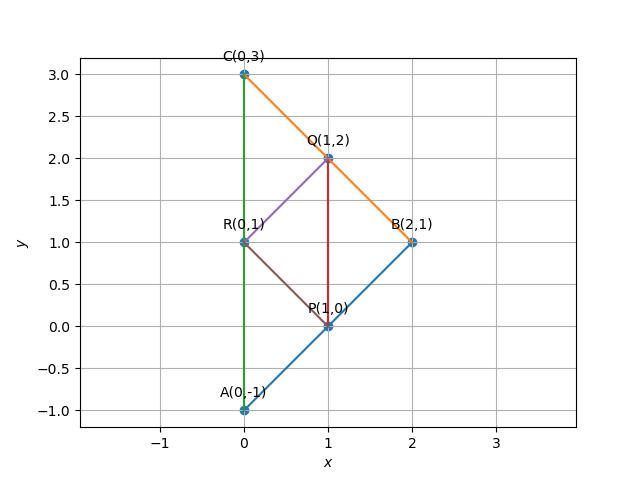
\includegraphics[width=\columnwidth]{chapters/10/7/3/3/figs/trigraph.png}
	\end{center}
\caption{}
\label{fig:10/7/3/3Fig}
\end{figure}


\item Find the area of the quadrilateral whose vertices, taken in order, are $(– 4, – 2), (– 3, – 5), (3, – 2)$  and $ (2, 3)$.
	\\
\solution
		\iffalse
\documentclass[12pt]{article}
\usepackage{graphicx}
%\documentclass[journal,12pt,twocolumn]{IEEEtran}
\usepackage[none]{hyphenat}
\usepackage{graphicx}
\usepackage{listings}
\usepackage[english]{babel}
\usepackage{graphicx}
\usepackage{caption} 
\usepackage{hyperref}
\usepackage{booktabs}
\def\inputGnumericTable{}
\usepackage{color}                                            %%
    \usepackage{array}                                            %%
    \usepackage{longtable}                                        %%
    \usepackage{calc}                                             %%
    \usepackage{multirow}                                         %%
    \usepackage{hhline}                                           %%
    \usepackage{ifthen}
\usepackage{array}
\usepackage{amsmath}   % for having text in math mode
\usepackage{listings}
\lstset{
language=tex,
frame=single, 
breaklines=true
}
  
%Following 2 lines were added to remove the blank page at the beginning
\usepackage{atbegshi}% http://ctan.org/pkg/atbegshi
\AtBeginDocument{\AtBeginShipoutNext{\AtBeginShipoutDiscard}}
%
%New macro definitions
\newcommand{\mydet}[1]{\ensuremath{\begin{vmatrix}#1\end{vmatrix}}}
\providecommand{\brak}[1]{\ensuremath{\left(#1\right)}}
\providecommand{\norm}[1]{\left\lVert#1\right\rVert}
\newcommand{\solution}{\noindent \textbf{Solution: }}
\newcommand{\myvec}[1]{\ensuremath{\begin{pmatrix}#1\end{pmatrix}}}
\let\vec\mathbf
\begin{document}
\begin{center}
\title{\textbf{Coordinate Geometry}}
\date{\vspace{-5ex}} %Not to print date automatically
\maketitle
\end{center}
\setcounter{page}{1}
\section*{10$^{th}$ Maths - Chapter 7}
This is Problem-4 from Exercise 7.3
\begin{enumerate}
\item Find the area of quadrilateral whose vertices, taken in order, are $\myvec{-4 \\ -2}, \myvec{-3\\-5}, \myvec{3\\-2}$ and $\myvec{2\\3}$.\\
	\solution 
\fi
		The input parameters for this problem are available in Table \eqref{tab:10/7/3/4}.
\begin{table}[ht!]\centering
%%%%%%%%%%%%%%%%%%%%%%%%%%%%%%%%%%%%%%%%%%%%%%%%%%%%%%%%%%%%%%%%%%%%%%
%%                                                                  %%
%%  This is the header of a LaTeX2e file exported from Gnumeric.    %%
%%                                                                  %%
%%  This file can be compiled as it stands or included in another   %%
%%  LaTeX document. The table is based on the longtable package so  %%
%%  the longtable options (headers, footers...) can be set in the   %%
%%  preamble section below (see PRAMBLE).                           %%
%%                                                                  %%
%%  To include the file in another, the following two lines must be %%
%%  in the including file:                                          %%
%%        \def\inputGnumericTable{}                                 %%
%%  at the beginning of the file and:                               %%
%%        \input{name-of-this-file.tex}                             %%
%%  where the table is to be placed. Note also that the including   %%
%%  file must use the following packages for the table to be        %%
%%  rendered correctly:                                             %%
%%    \usepackage[latin1]{inputenc}                                 %%
%%    \usepackage{color}                                            %%
%%    \usepackage{array}                                            %%
%%    \usepackage{longtable}                                        %%
%%    \usepackage{calc}                                             %%
%%    \usepackage{multirow}                                         %%
%%    \usepackage{hhline}                                           %%
%%    \usepackage{ifthen}                                           %%
%%  optionally (for landscape tables embedded in another document): %%
%%    \usepackage{lscape}                                           %%
%%                                                                  %%
%%%%%%%%%%%%%%%%%%%%%%%%%%%%%%%%%%%%%%%%%%%%%%%%%%%%%%%%%%%%%%%%%%%%%%



%%  This section checks if we are begin input into another file or  %%
%%  the file will be compiled alone. First use a macro taken from   %%
%%  the TeXbook ex 7.7 (suggestion of Han-Wen Nienhuys).            %%
\def\ifundefined#1{\expandafter\ifx\csname#1\endcsname\relax}


%%  Check for the \def token for inputed files. If it is not        %%
%%  defined, the file will be processed as a standalone and the     %%
%%  preamble will be used.                                          %%
\ifundefined{inputGnumericTable}

%%  We must be able to close or not the document at the end.        %%
 \def\gnumericTableEnd{\end{document}}


%%%%%%%%%%%%%%%%%%%%%%%%%%%%%%%%%%%%%%%%%%%%%%%%%%%%%%%%%%%%%%%%%%%%%%
%%                                                                  %%
%%  This is the PREAMBLE. Change these values to get the right      %%
%%  paper size and other niceties.                                  %%
%%                                                                  %%
%%%%%%%%%%%%%%%%%%%%%%%%%%%%%%%%%%%%%%%%%%%%%%%%%%%%%%%%%%%%%%%%%%%%%%

 \documentclass[12pt%
     %,landscape%
                    ]{report}
       \usepackage[latin1]{inputenc}
       \usepackage{fullpage}
       \usepackage{color}
       \usepackage{array}
       \usepackage{longtable}
       \usepackage{calc}
       \usepackage{multirow}
       \usepackage{hhline}
       \usepackage{ifthen}

 \begin{document}


%%  End of the preamble for the standalone. The next section is for %%
%%  documents which are included into other LaTeX2e files.          %%
\else

%%  We are not a stand alone document. For a regular table, we will %%
%%  have no preamble and only define the closing to mean nothing.   %%
    \def\gnumericTableEnd{}

%%  If we want landscape mode in an embedded document, comment out  %%
%%  the line above and uncomment the two below. The table will      %%
%%  begin on a new page and run in landscape mode.                  %%
%       \def\gnumericTableEnd{\end{landscape}}
%       \begin{landscape}


%%  End  theoelse clause for this file being \input.              %%
\fi

%%%%%%%%%%%%%%%%%%%%%%%%%%%%%%%%%%%%%%%%%%%%%%%%%%%%%%%%%%%%%%%%%%%%%%
%%                                                                  %%
%%  The rest is the gnumeric table, except for the closing          %%
%%  statement. Changes below will alter the table's appearance.     %%
%%                                                                  %%
%%%%%%%%%%%%%%%%%%%%%%%%%%%%%%%%%%%%%%%%%%%%%%%%%%%%%%%%%%%%%%%%%%%%%%

\providecommand{\gnumericmathit}[1]{#1} 
%%  Uncomment the next line if you would like your numbers to be in %%
%%  italics if they are italizised in the gnumeric table.           %%
%\renewcommand{\gnumericmathit}[1]{\mathit{#1}}
\providecommand{\gnumericPB}[1]%
{\let\gnumericTemp=\\#1\let\\=\gnumericTemp\hspace{0pt}}
 \ifundefined{gnumericTableWidthDefined}
        \newlength{\gnumericTableWidth}
        \newlength{\gnumericTableWidthComplete}
        \newlength{\gnumericMultiRowLength}
        \global\def\gnumericTableWidthDefined{}
 \fi
%% The following setting protects this code from babel shorthands.  %%
 \ifthenelse{\isundefined{\languageshorthands}}{}{\languageshorthands{english}}
%%  The default table format retains the relative column widths of  %%
%%  gnumeric. They can easily be changed to c, r or l. In that case %%
%%  you may want to comment out the next line and uncomment the one %%
%%  thereafter                                                      %%
\providecommand\gnumbox{\makebox[0pt]}
%%\providecommand\gnumbox[1][]{\makebox}

%% to adjust positions in multirow situations                       %%
\setlength{\bigstrutjot}{\jot}
\setlength{\extrarowheight}{\doublerulesep}

%%  The \setlongtables command keeps column widths the same across  %%
%%  pages. Simply comment out next line for varying column widths.  %%
\setlongtables

\setlength\gnumericTableWidth{%
 53pt+%
 53pt+%
 82pt+%
 53pt+%
0pt}
\def\gumericNumCols{4}
\setlength\gnumericTableWidthComplete{\gnumericTableWidth+%
         \tabcolsep*\gumericNumCols*2+\arrayrulewidth*\gumericNumCols}
\ifthenelse{\lengthtest{\gnumericTableWidthComplete > \linewidth}}%
         {\def\gnumericScale{1*\ratio{\linewidth-%
                        \tabcolsep*\gumericNumCols*2-%
                        \arrayrulewidth*\gumericNumCols}%
{\gnumericTableWidth}}}%
{\def\gnumericScale{1}}

%%%%%%%%%%%%%%%%%%%%%%%%%%%%%%%%%%%%%%%%%%%%%%%%%%%%%%%%%%%%%%%%%%%%%%
%%                                                                  %%
%% The following are the widths of the various columns. We are      %%
%% defining them here because then they are easier to change.       %%
%% Depending on the cell formats we may use them more than once.    %%
%%                                                                  %%
%%%%%%%%%%%%%%%%%%%%%%%%%%%%%%%%%%%%%%%%%%%%%%%%%%%%%%%%%%%%%%%%%%%%%%

\ifthenelse{\isundefined{\gnumericColA}}{\newlength{\gnumericColA}}{}\settowidth{\gnumericColA}{\begin{tabular}{@{}p{53pt*\gnumericScale}@{}}x\end{tabular}}
\ifthenelse{\isundefined{\gnumericColB}}{\newlength{\gnumericColB}}{}\settowidth{\gnumericColB}{\begin{tabular}{@{}p{53pt*\gnumericScale}@{}}x\end{tabular}}
\ifthenelse{\isundefined{\gnumericColC}}{\newlength{\gnumericColC}}{}\settowidth{\gnumericColC}{\begin{tabular}{@{}p{82pt*\gnumericScale}@{}}x\end{tabular}}
\ifthenelse{\isundefined{\gnumericColD}}{\newlength{\gnumericColD}}{}\settowidth{\gnumericColD}{\begin{tabular}{@{}p{53pt*\gnumericScale}@{}}x\end{tabular}}

\begin{center}
\begin{tabular}[c]{%
 b{\gnumericColA}%
 b{\gnumericColB}%
 b{\gnumericColC}%
 b{\gnumericColD}%
 }

%%%%%%%%%%%%%%%%%%%%%%%%%%%%%%%%%%%%%%%%%%%%%%%%%%%%%%%%%%%%%%%%%%%%%%
%%  The longtable options. (Caption, headers... see Goosens, p.124) %%
% \caption{The Table Caption.}             \\ %
% \hline % Across the top of the table.
%%  The rest of these options are table rows which are placed on    %%
%%  the first, last or every page. Use \multicolumn if you want.    %%

%%  Header for the first page.                                      %%
% \multicolumn{4}{c}{The First Header} \\ \hline 
% \multicolumn{1}{c}{colTag} %Column 1
% &\multicolumn{1}{c}{colTag} %Column 2
% &\multicolumn{1}{c}{colTag} %Column 3
% &\multicolumn{1}{c}{colTag} \\ \hline %Last column
% \endfirsthead

%%  The running header definition.                                  %%
% \hline
% \multicolumn{4}{l}{\ldots\small\slshape continued} \\ \hline
% \multicolumn{1}{c}{colTag} %Column 1
% &\multicolumn{1}{c}{colTag} %Column 2
% &\multicolumn{1}{c}{colTag} %Column 3
% &\multicolumn{1}{c}{colTag} \\ \hline %Last column
% \endhead

%%  The running footer definition.                                  %%
% \hline
% \multicolumn{4}{r}{\small\slshape continued\ldots} \\
% \endfoot

%%  The ending footer definition.                                   %%
% \multicolumn{4}{c}{That's all folks} \\ \hline 
% \endlastfoot
%%%%%%%%%%%%%%%%%%%%%%%%%%%%%%%%%%%%%%%%%%%%%%%%%%%%%%%%%%%%%%%%%%%%%%

\hhline{|-|-|-~}
  \multicolumn{1}{|p{\gnumericColA}|}%
 {\gnumericPB{\centering}\gnumbox{\textbf{Symbol}}}
 &\multicolumn{1}{p{\gnumericColB}|}%
 {\gnumericPB{\centering}\gnumbox{\textbf{Value}}}
 &\multicolumn{1}{p{\gnumericColC}|}%
 {\gnumericPB{\centering}\gnumbox{\textbf{Description}}}
 &
\\
\hhline{|---|~}
  \multicolumn{1}{|p{\gnumericColA}|}%
 {\gnumericPB{\centering}\gnumbox{$\vec{A}$}}
 &\multicolumn{1}{p{\gnumericColB}|}%
 {\gnumericPB{\centering}\gnumbox{$\myvec{-4\\-2}$}}
 &\multicolumn{1}{p{\gnumericColC}|}%
 {\gnumericPB{\centering}\gnumbox{First point}}
 &
\\
\hhline{|---|~}
  \multicolumn{1}{|p{\gnumericColA}|}%
 {\gnumericPB{\centering}\gnumbox{$\vec{B}$}}
 &\multicolumn{1}{p{\gnumericColB}|}%
 {\gnumericPB{\centering}\gnumbox{$\myvec{-3\\-5}$}}
 &\multicolumn{1}{p{\gnumericColC}|}%
 {\gnumericPB{\centering}\gnumbox{Second point}}
 &
\\
\hhline{|---|~}
  \multicolumn{1}{|p{\gnumericColA}|}%
 {\gnumericPB{\centering}\gnumbox{$\vec{C}$}}
 &\multicolumn{1}{p{\gnumericColB}|}%
 {\gnumericPB{\centering}\gnumbox{$\myvec{3\\-2}$}}
 &\multicolumn{1}{p{\gnumericColC}|}%
 {\gnumericPB{\centering}\gnumbox{Third point}}
 &
\\

\hhline{|---|~}
  \multicolumn{1}{|p{\gnumericColA}|}%
 {\gnumericPB{\centering}\gnumbox{$\vec{D}$}}
 &\multicolumn{1}{p{\gnumericColB}|}%
 {\gnumericPB{\centering}\gnumbox{$\myvec{2\\3}$}}
 &\multicolumn{1}{p{\gnumericColC}|}%
 {\gnumericPB{\centering}\gnumbox{Fourth point}}
 &
\\
\hhline{|-|-|-|~}
\end{tabular}
 \end{center}

\ifthenelse{\isundefined{\languageshorthands}}{}{\languageshorthands{\languagename}}
%\gnumericTableEndf

\caption{}
\label{tab:10/7/3/4}	
\end{table}
By joining $\vec{B}$ to $\vec{D}$, two triangles $\vec{A}\vec{B}\vec{D}$ and $\vec{B}\vec{C}\vec{D}$ are obtained.
Since
\begin{align}
	\vec{A}- \vec{B} &= \myvec{-4\\-2\\}-\myvec{-3\\-5\\}=\myvec{-1\\3\\}\label{eq:chapters/10/7/3/4/2}\\
	  \vec{A}- \vec{D} &= \myvec{-4\\-2\\}-\myvec{2\\3\\}=\myvec{-6\\-5\\}\label{eq:chapters/10/7/3/4/3}
  \end{align}
  \begin{align}
	  ar(ABD)&=\frac{1}{2} \norm{\brak{\vec{A}-\vec{B}}  \times 
   \brak{\vec{A}- \vec{D}}} \label{eq:chapters/10/7/3/4/1} 
   \\
	  &=	\frac{1}{2}\mydet{-1 & 3\\-6 & -5}  
	=	\frac{23}{2}
\end{align}
upon substituting the values of \eqref{eq:chapters/10/7/3/4/2} and \eqref{eq:chapters/10/7/3/4/3} in \eqref{eq:chapters/10/7/3/4/1}.
Similarly,
\begin{align}
	\vec{B}- \vec{C} &= \myvec{-3\\-5\\}-\myvec{3\\-2\\}=\myvec{-6\\-5\\}\label{eq:chapters/10/7/3/4/6} \\
	  \vec{B}- \vec{D} &= \myvec{-3\\-5\\}-\myvec{2\\3\\}=\myvec{-3\\-8\\}\label{eq:chapters/10/7/3/4/7} 
  \end{align}
  yielding
  \begin{align}
	  ar(BCD)&=\frac{1}{2} \norm{\brak{\vec{B}-\vec{C}}  \times 
   \brak{\vec{B}- \vec{D}}} \label{eq:chapters/10/7/3/4/5}
   \\
	  &=	\frac{1}{2}\mydet{-6 & -3\\-5 & -8}  
	=	\frac{33}{2}
\end{align}
	upon 	substituting the values of \eqref{eq:chapters/10/7/3/4/6} and \eqref{eq:chapters/10/7/3/4/7} in \eqref{eq:chapters/10/7/3/4/5}
		Thus, 
\begin{align}
	ar(ABCD)&=  ar(ABD) +  ar(BCD)
	= 28
\end{align}
See Fig. 
\ref{fig:chapters/10/7/3/4/Fig1}
\begin{figure}[!h]
 \begin{center}
  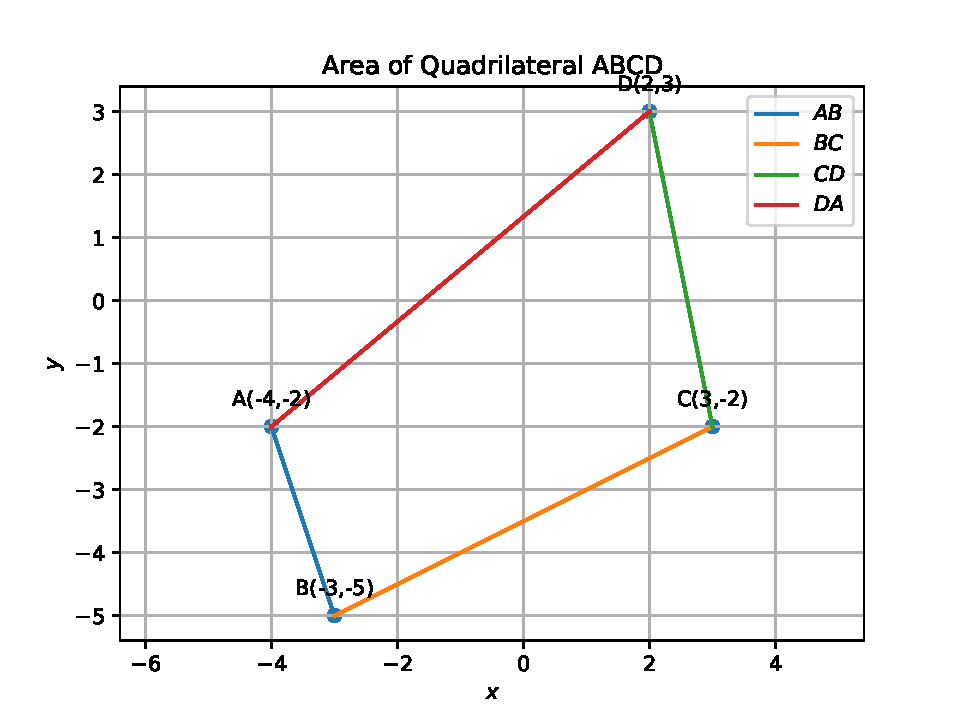
\includegraphics[width=\columnwidth]{chapters/10/7/3/4/figs/fig.pdf}
 \end{center}
\caption{}
\label{fig:chapters/10/7/3/4/Fig1}
\end{figure}


\item Verify that a median of a triangle divides it into two triangles of equal areas for $\triangle ABC$ whose vertices are $\vec{A}(4, -6), \vec{B}(3, 2), \text{ and } \vec{C}(5, 2)$. 
		\label{10/7/3/5}
		\\
\solution
		\iffalse
\documentclass[12pt]{article}
\usepackage{graphicx}
\usepackage[none]{hyphenat}
\usepackage{graphicx}
\usepackage{listings}
\usepackage[english]{babel}
\usepackage{graphicx}
\usepackage{caption} 
\usepackage{booktabs}
\usepackage{array}
\usepackage{amssymb} % for \because
\usepackage{amsmath}   % for having text in math mode
\usepackage{extarrows} % for Row operations arrows
\usepackage{listings}
\usepackage[utf8]{inputenc}
\lstset{
  frame=single,
  breaklines=true
}
\usepackage{hyperref}
  
%Following 2 lines were added to remove the blank page at the beginning
\usepackage{atbegshi}% http://ctan.org/pkg/atbegshi
\AtBeginDocument{\AtBeginShipoutNext{\AtBeginShipoutDiscard}}


%New macro definitions
\newcommand{\mydet}[1]{\ensuremath{\begin{vmatrix}#1\end{vmatrix}}}
\providecommand{\brak}[1]{\ensuremath{\left(#1\right)}}
\newcommand{\solution}{\noindent \textbf{Solution: }}
\newcommand{\myvec}[1]{\ensuremath{\begin{pmatrix}#1\end{pmatrix}}}
\providecommand{\norm}[1]{\left\lVert#1\right\rVert}
\providecommand{\abs}[1]{\left\vert#1\right\vert}
\let\vec\mathbf

\begin{document}

\begin{center}
\title{\textbf{VECTORS}}
\date{\vspace{-5ex}} %Not to print date automatically
\maketitle
\end{center}

\section{10$^{th}$ Maths - EXERCISE-7.3}

\begin{enumerate}
\item That a median of a triangle divides it into two triangles  of equal areas. verify this result for $\triangle ABC$ whose vertices are $\vec{A}(4,-6),\vec{B}(3,-2)\text{ and }\vec{C}(5,2)$.
\end{enumerate}

\section{SOLUTION}
Given points are
\begin{align}
\vec{A}=\myvec{4\\ -6} ,
\vec{B}=\myvec{3\\ -2} ,
\vec{C}=\myvec{5\\ 2}
\end{align}
\fi
The median of the triangle 
\begin{align}
\vec{D}&=\frac{\vec{B}+\vec{C}}{2}\\
&=\myvec{4\\ 0}
\end{align}
Since 
\begin{align}
	\vec{A}- \vec{B} &= \myvec{4\\ -6}-\myvec{3\\ -2}=\myvec{1\\ -4}\label{eq:10/7/3/5/7}\\
	  \vec{A}- \vec{D} &= \myvec{4\\ -6}-\myvec{4\\ 0}=\myvec{0\\ -6}\label{eq:10/7/3/5/8}
  \end{align}
 \begin{align}
  ar(ABD)&=\frac{1}{2} \norm{\brak{\vec{A}-\vec{B}}  \times 
   \brak{\vec{A}- \vec{D}}} \label{eq:10/7/3/5/6} 
   \\
&=\frac{1}{2}\mydet{1 & 0\\-4 & -6}
	       =3	
\end{align}
upon
Substituting from \eqref{eq:10/7/3/5/7} and \eqref{eq:10/7/3/5/8} in \eqref{eq:10/7/3/5/6}.
		Similarly, 
\begin{align}
	\vec{A}- \vec{C} &= \myvec{4\\ -6}-\myvec{5\\ 2}=\myvec{-1\\ -8}\label{eq:10/7/3/5/13} \\
	  \vec{A}- \vec{D} &= \myvec{4\\ -6}-\myvec{4\\ 0}=\myvec{0\\ -6}\label{eq:10/7/3/5/14} 
  \end{align}
  yielding
  \begin{align}
  ar(ACD)&=\frac{1}{2} \norm{\brak{\vec{A}-\vec{C}}  \times 
   \brak{\vec{A}- \vec{D}}} \label{eq:10/7/3/5/12}
   \\
	&=\frac{1}{2}\mydet{-1 & 0\\-8 & -6}= 3
\end{align}
upon substituting from \eqref{eq:10/7/3/5/13} and \eqref{eq:10/7/3/5/14} in \eqref{eq:10/7/3/5/12}.
Thus,
\begin{align}
ar(ABD)=ar(ACD)
\end{align}
See Fig. 
\ref{fig:10/7/3/5/}.
\begin{figure}[h!]
\centering
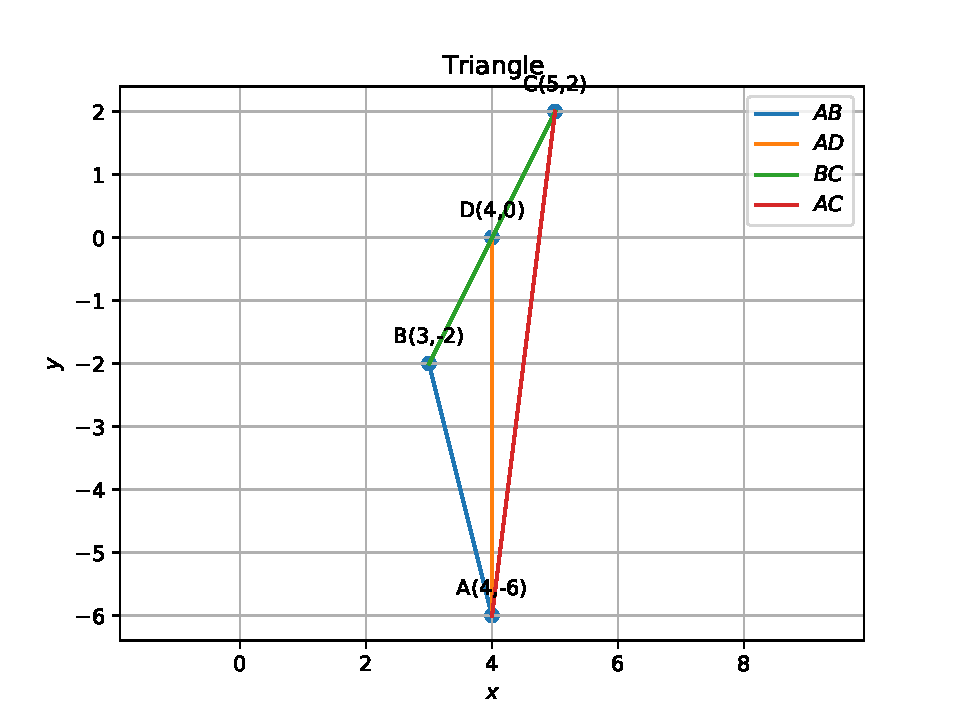
\includegraphics[width=\columnwidth]{chapters/10/7/3/5/figs/fig.pdf}
\caption{}
\label{fig:10/7/3/5/}
\end{figure} 


\item Find the area of region bounded by the triangle whose
	vertices are $(1, 0), (2, 2) \text{ and } (3, 1)$. 
\item Find the area of region bounded by the triangle whose vertices
	are $(– 1, 0), (1, 3) \text{ and } (3, 2)$. 

\item Find the area of the $\triangle ABC$, coordinates of whose vertices are $\vec{A}(2, 0), \vec{B}(4, 5), \text{ and } \vec{C}(6, 3)$.

\end{enumerate}


